\section{Results III: the decision system under a cost criterion}\label{sec:system}

The two laws above constrain the components; this section reports the system they
were meant to serve, so that the efficiency questions are anchored to a decision
problem rather than to a benchmark.

\subsection{Supervised baselines and the cost of a second stage}

\begin{table}[t]
\centering
\begin{tabular}{lrrrrr}
\toprule
system & AUC-PR & AUC-ROC & R@FPR$=1\%$ & loss & cost/tx \\
\midrule
linear (logistic) & 0.1874 & 0.7573 & 14.0\% & 9{,}299 & 1.00 \\
GBDT gate & 0.4551 & 0.8664 & 38.6\% & 6{,}653 & 1.00 \\
GBDT strong & 0.4691 & 0.8734 & 40.2\% & 6{,}580 & 20.00 \\
cascade (gate+strong) & 0.4711 & 0.8729 & 39.5\% & 6{,}552 & 19.08 \\
\bottomrule
\end{tabular}

\caption{Held-out performance on \DatasetIeee{} with \MainFeatures{} predictors,
\MainTrainRows{} training rows and \MainTestRows{} test rows. The operating point
is chosen once on validation at a $1\%$ false-positive rate. Cost per transaction
is a proxy counting the second stage as twenty times the first, not a measured
latency. Data: \texttt{s5\_baselines/main\_table.json}.}
\label{tab:main}
\end{table}

Table~\ref{tab:main} reports \Nsys{} systems. The linear model reaches AUC-PR
\AucPrLinear, the gradient-boosted gate \AucPrGbdt, a stronger gradient-boosted
second stage \AucPrStrong, and the cascade \AucPrCascade. The cascade buys
$+\PermDeltaCvG$ AUC-PR over the gate alone at a proxy cost of \CostCascade{}
against \CostStrong{} for running the strong model on everything, with an upgrade
rate of \UpgradeRate\%. The gain is small but not attributable to noise: the paired
permutation test gives $p<10^{-3}$ and the entity-cluster bootstrap interval
excludes zero (\PermCiLoCvG--\PermCiHiCvG), while the recall-at-$1\%$-FPR interval
includes zero, so the ranking improvement does not translate into a better
operating point. We report both.

The comparison that matters statistically is the one between the linear model and
the gate: $\Delta$AUC $=\DelongDelta$ (95\% CI \DelongCiLo--\DelongCiHi,
$z=\DelongZ$), with \McNemarDiscordant{} discordant pairs under McNemar
($b=\McNemarB$, $c=\McNemarC$, $p=\McNemarP$). Across \SeedN{} independent
retraining seeds the gate's AUC-PR is \SeedMean$\pm$\SeedSd, and the a-priori
power calculation says that \RequiredSeeds{} seeds would be needed to resolve a
difference of the size we observe at $80\%$ power. We therefore report the effect
size and the interval rather than a bare $p$-value, and we do not claim a
difference between systems whose intervals overlap.

\subsection{Cost sensitivity}

\begin{table}[t]
\centering
\begin{tabular}{rrrrr}
\toprule
$c_{\mathrm{FN}}/c_{\mathrm{FP}}$ & threshold & cost/tx & recall & FPR \\
\midrule
1 & 0.3058 & 0.0292 & 33.5\% & 0.58\% \\
2 & 0.2322 & 0.0527 & 38.3\% & 0.93\% \\
5 & 0.1531 & 0.1208 & 42.5\% & 1.95\% \\
10 & 0.0800 & 0.2124 & 54.5\% & 5.27\% \\
20 & 0.0370 & 0.3803 & 67.9\% & 15.79\% \\
50 & 0.0195 & 0.6403 & 79.4\% & 28.55\% \\
100 & 0.0096 & 0.7917 & 92.3\% & 53.57\% \\
\bottomrule
\end{tabular}

\caption{Cost sensitivity on \DatasetIeee{} test rows. The threshold is chosen on
validation for each cost ratio and applied once to test. Data:
\texttt{s4\_stats/cost\_sensitivity.json}.}
\label{tab:cost}
\end{table}

Table~\ref{tab:cost} and Figure~\ref{fig:cost} sweep the ratio
$c_{\mathrm{FN}}/c_{\mathrm{FP}}$ from $1$ to \CostRatioMax{} and re-select the
threshold on validation each time. Expected cost per transaction rises from
\CostAtOne{} to \CostAtHundred{} as the ratio increases, which is expected: a
higher relative cost of a missed fraud buys recall with false alarms, and recall
moves from \RecallAtOne\% to \RecallAtHundred\% while the false-positive rate moves
to \FprAtHundred\%. The useful observation is that the threshold responds smoothly
and monotonically, so the deployed operating point can be audited against a stated
cost ratio instead of being fixed by convention. It also makes the insufficiency of
a single number concrete: the same model is a different system at ratio $1$ and at
ratio $100$.

\begin{figure}[t]
\centering
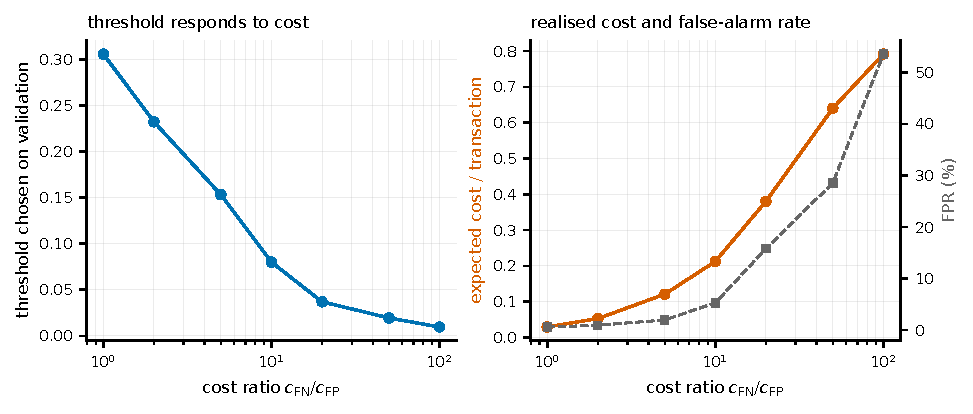
\includegraphics[width=\textwidth]{fig6_cost.pdf}
\caption{Threshold selected on validation (left) and realised test cost with the
false-positive rate (right) as the relative cost of a missed fraud increases. Data:
\texttt{s4\_stats/cost\_sensitivity.json}.}
\label{fig:cost}
\end{figure}

\subsection{Where the model transfers, and where it does not}

On \DatasetBaf{} the same pipeline with \BafFeatures{} predictors reaches AUC-PR
\BafAucPr{} and AUC-ROC \BafAucRoc{} at \BafRecall\% recall at a $1\%$ false-positive
rate. We report the number without enthusiasm and with two caveats. The dataset is
source-declared synthetic, so this is a transfer check rather than external
validation; and its base rate is lower than \DatasetIeee{}'s, so the two AUC-PR
values are not directly comparable.

Within the held-out periods of \DatasetIeee{} the AUC-PR moves by \IeeeDrift{}
between the first and last temporal slice, i.e. it is essentially flat. On
\DatasetBaf{} it moves by \BafDrift{}, and the move is confounded: the fraud
prevalence rises from \BafPrevLo\% to \BafPrevHi\% over the same interval, and
AUC-PR is prevalence-sensitive. We therefore do not interpret the second number as
evidence of improving robustness, and we record the confound rather than the
headline.

Fairness is reported as equalised-odds gaps \cite{hardt2016equality} over the
\FairAttrs{} attributes the dataset provides. The largest true-positive-rate gap
is \FairTprGap{} on \texttt{\FairAttr} across \FairGroups{} groups, with a
false-positive-rate gap of \FairFprGap; the smallest true-positive-rate gap among
the attributes is \FairMinTprGap. These gaps are a property of a single threshold
on a single dataset and we make no claim about their cause.

\subsection{Two interventions that did not help}

Calibration is the standard remedy for scores that are used as probabilities.
Fitting Platt scaling on validation and evaluating on test moves the Brier score
from \BrierPre{} to \BrierPost{} and the expected calibration error from \EcePre{}
to \EcePost; the intervention does not reduce the Brier score
(\texttt{platt\_reduces\_brier}, whose value here is \PlattImproves). The
gradient-boosted scores were already close to calibrated at this operating point,
so the honest report is a null result, and we keep it rather than dropping the
comparison.

The learning curve over labelled-set sizes from the smallest to the largest size
we evaluate moves AUC-PR from \CurveSmallAucPr{} to \CurveLargeAucPr{} across
\CurveSizes{} sizes. At the smallest size a minority floor has to be enforced,
because a uniform draw at a $3.5\%$ rate contains no positive example at all, so
the left end of the curve is an artefact of the apparatus rather than a scientific
finding.
We report the artefact because a crossover claim at that size would otherwise look
like a result. The field ladder from \LadderSmall{} to \LadderLarge{} fields moves
AUC-PR from \LadderSmallestAucPr{} to \LadderLargestAucPr, which is the expected
saturating shape and confirms that the feature budget used elsewhere in the paper
is not the binding constraint.

\subsection{What verifiability costs}

If a decision must be auditable, the audit itself has a cost, and it is fair to
state it in the same currency as the rest. A commitment-and-challenge protocol
commits to each decision, anchors a batch root, and answers a random challenge by
recomputation. We compile a registry contract with \SolcVer{} and execute it on a
local EVM: one per-transaction log commitment costs \GasPerTx{} gas (standard
deviation \GasPerTxSd), one batch root costs \GasBatch, and verifying one inclusion
proof of depth \MerkleDepth{} costs \GasVerify. Anchoring \GasBatchSize{}
transactions in one root instead of individually reduces the anchoring cost by
\GasSavingPct\%. Deployment costs \GasDeploy{} gas and is amortised.

Two limits are stated rather than papered over. First, this is a local EVM: the
numbers are receipts from executed transactions rather than a public-network
market quote, and the pricing constants are labelled as reference values that
rescale the dollar figure linearly. Second, the soundness argument for the
challenge protocol is game-theoretic, not hardware-rooted: the escape probability
of an adversary who cheats on a fraction $f$ of records falls geometrically in the
challenge rate, and a predictable challenge source destroys the guarantee
entirely. Hardware attestation \cite{costan2016sgx} and proof-of-learning
\cite{jia2021proof} would replace that assumption. Neither is measurable on this
device: the attestation unit is recorded as blocked, with the command that would
unblock it, and the proof-carrying variant was not attempted for the same reason.
We estimate neither, and no number in this paper depends on them.
